\section{The kernel trick}

\begin{frame}\frametitle{\secname}

Representing a non-linear transformation using inner products of the data:
\begin{equation}
 \label{eq:trick}
      \vec{\phi}_{(\vec{x})}^\top 
		\vec{\phi}_{(\vec{x}')} = 
      k(\vec{x}, \vec{x}')
\end{equation}
    
where $k(\vec{x}, \vec{x}')$ is a kernel function applied 
to any two observations.

\end{frame}

\subsection{The Kernel matrix}

\begin{frame}\frametitle{\subsecname}

Applying the kernel function to \emph{each} pair in our dataset; \\
$\vec x^{(\alpha)}$ and $\vec{x}^{(\beta)}$ 
with $\alpha, \beta = 1, \ldots, p$ yields the scalar $K_{\alpha \beta}$. 
Storing all scalars $K_{\alpha \beta} \; \forall (\alpha,\beta)$ yields 
the un-normalized kernel matrix $\widetilde {\vec K}=\{K_{\alpha \beta}\}$:

\begin{equation}
\widetilde {\vec K} = 
\rmat{
K_{11} & K_{12} & \ldots & K_{1p} \\
K_{21} & K_{12} & \ldots & K_{2p} \\
\vdots & & \ddots\\
K_{p1} & & & K_{pp}
}
\end{equation}

$\vec K$ (without the ``\textasciitilde'') denotes the normalized or ``centered'' kernel matrix. \notesonly{cf. \sectionref{sec:centerkernel} on why and how to center the Kernel matrix.}

\question{What is the dimensionality of $\widetilde {\vec K}$?}

\end{frame}

\subsubsection{Properties of the Kernel matrix}

\begin{frame}\frametitle{\subsubsecname}

\begin{block}{From Mercer's theorem}
Every positive semidefinite kernel $k$ corresponds to a scalar product in
some metric feature space.
\end{block}

\end{frame}

\subsubsection{The Radial Basis function (RBF) Kernel}

\begin{frame}\frametitle{The Radial Basis function (RBF) }

\notesonly{The radial basis function (RBF) as depicted in \figref{fig:rbf} is a popular choice for a kernel. It is defined as:}

\begin{equation}
	k_{(\vec{x},\vec{x}')} = \exp \bigg\{ -\frac{ \big( \vec{x} - \vec{x}' 
					\big)^2 }{ 2 \sigma^2 } \bigg\}
\end{equation}

where $\sigma$ is referred to as the width of the kernel.

\begin{figure}[ht]
     \centering
     \savebox{\imagebox}{
	 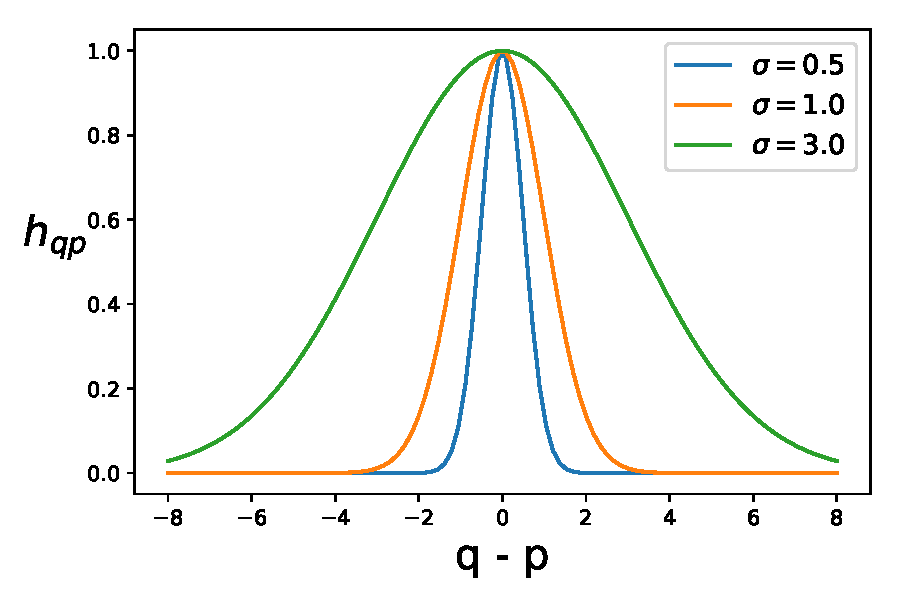
\includegraphics[width=\slidesonly{0.45}\notesonly{0.35}\textwidth]{img/guassian_function_1d}}%
     \begin{subfigure}[t]{\slidesonly{0.45}\notesonly{0.35}\textwidth}
         \centering
         \usebox{\imagebox}% Place largest image
         \caption{for data in 1D}
         \label{fig:quadratic}
     \end{subfigure}
     \hspace{2mm}
     \begin{subfigure}[t]{\slidesonly{0.45}\notesonly{0.35}\textwidth}
         \centering
         \raisebox{\dimexpr.5\ht\imagebox-.5\height}{% Raise smaller image into place
         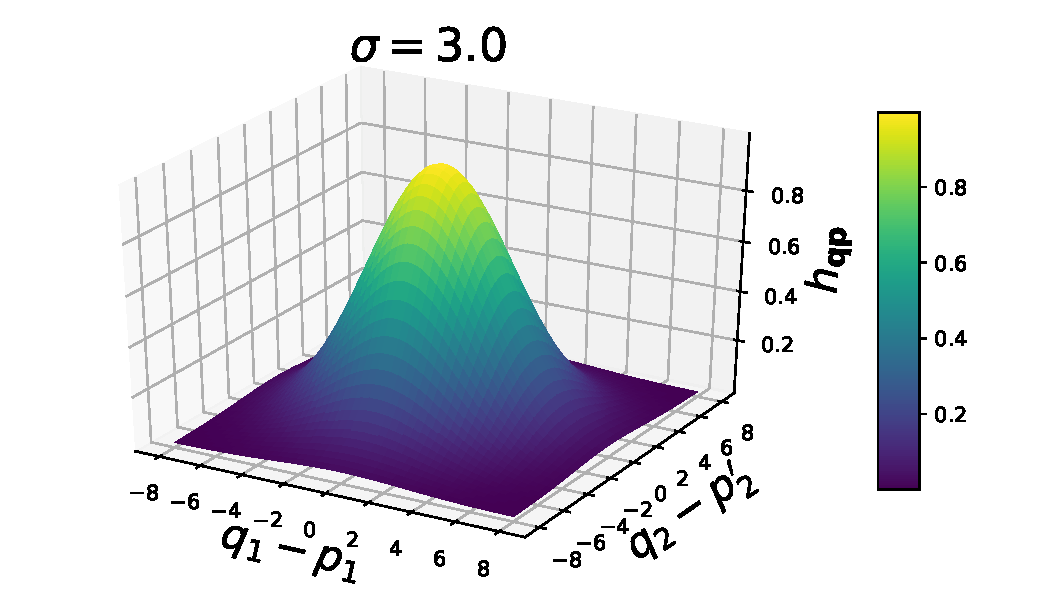
\includegraphics[width=0.99\textwidth]{img/guassian_function_2d_3Dview}
         }
         \caption{for data in 2D}
         \label{fig:linear}
     \end{subfigure}
     \mode<article>{
     \caption{The Gaussian kernel function}
     }
	 \label{fig:rbf}
\end{figure}

\end{frame}

\begin{frame}\frametitle{The RBF Kernel}

\slidesonly{
Applied to all pairs\\

\begin{minipage}{0.4\textwidth}

\only<1>{
\begin{equation}
	k_{(\vec{x},\vec{x}')} = \exp \bigg\{ -\frac{ \big( \vec{x} - \vec{x}' 
					\big)^2 }{ 2 \sigma^2 } \bigg\}
\end{equation}
}
\only<2>{
         \includegraphics[width=0.8\textwidth]{img/points_rbf}
}
\only<3>{
         \includegraphics[width=0.8\textwidth]{img/points_rbf_rot_transl}
}


\end{minipage}
\begin{minipage}{0.5\textwidth}
         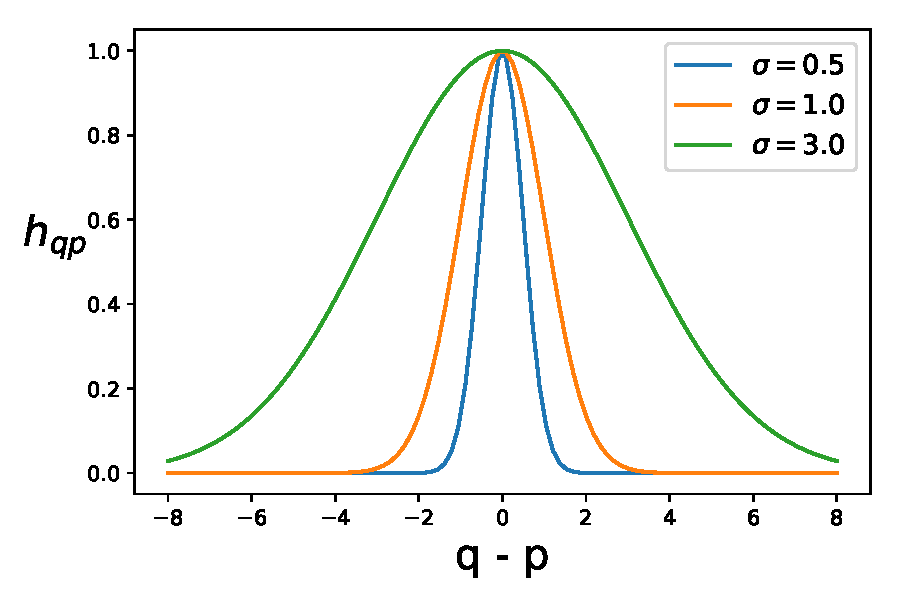
\includegraphics[width=0.99\textwidth]{img/guassian_function_1d}
\end{minipage}

}

\pause

\visible<2->{
\question{For an RBF kernel, is $K_{\alpha \beta}$ sensitive to translation and rotation of the input data?}
}

\mode<article>{
\begin{center}
	\includegraphics[width=0.2\textwidth]{img/points_rbf_rot_transl}
    \captionof{figure}{Rotation and translation of the input data}     
\end{center}

}


\pause

- No.\notesonly{ For an RBF Kernel, $K_{\alpha \beta}$ is the pairwise relation between two observations. 
Rotating the data or translating it will result in the same $K_{\alpha \beta}$.}
However, scaling the data while keeping the kernel width fixed would produce a different $K_{\alpha \beta}$.

\end{frame}


